\documentclass[tikz]{standalone}
\usepackage{ifthen}
\usepackage{pgfplots}
\pgfplotsset{compat=1.18}
\usepackage{physics}
\usepackage{siunitx}
\usepackage{tikz}
\usepackage{tikz-3dplot}
\usepackage{xcolor}
\usetikzlibrary{calc, angles, quotes, intersections}

% Tikz styles
\tikzset{axis/.style={thick, -latex}}
\tikzset{vec/.style={thick, blue}}
\tikzset{unitvec/.style={thick, red, -latex}}

\colorlet{wavecol}{orange!35!black}
\colorlet{freqcol}{green!25!black}
\colorlet{radarcol}{green!80!black!70}
\colorlet{ircol}{red!80!black!70}
\colorlet{enercol}{blue!35!black}
\pgfdeclareverticalshading{rainbow}{100bp}{
  color(0bp)=(red); color(25bp)=(red); color(35bp)=(yellow);
  color(45bp)=(green); color(55bp)=(cyan); color(65bp)=(blue);
  color(75bp)=(violet); color(100bp)=(violet)
}

\begin{document}

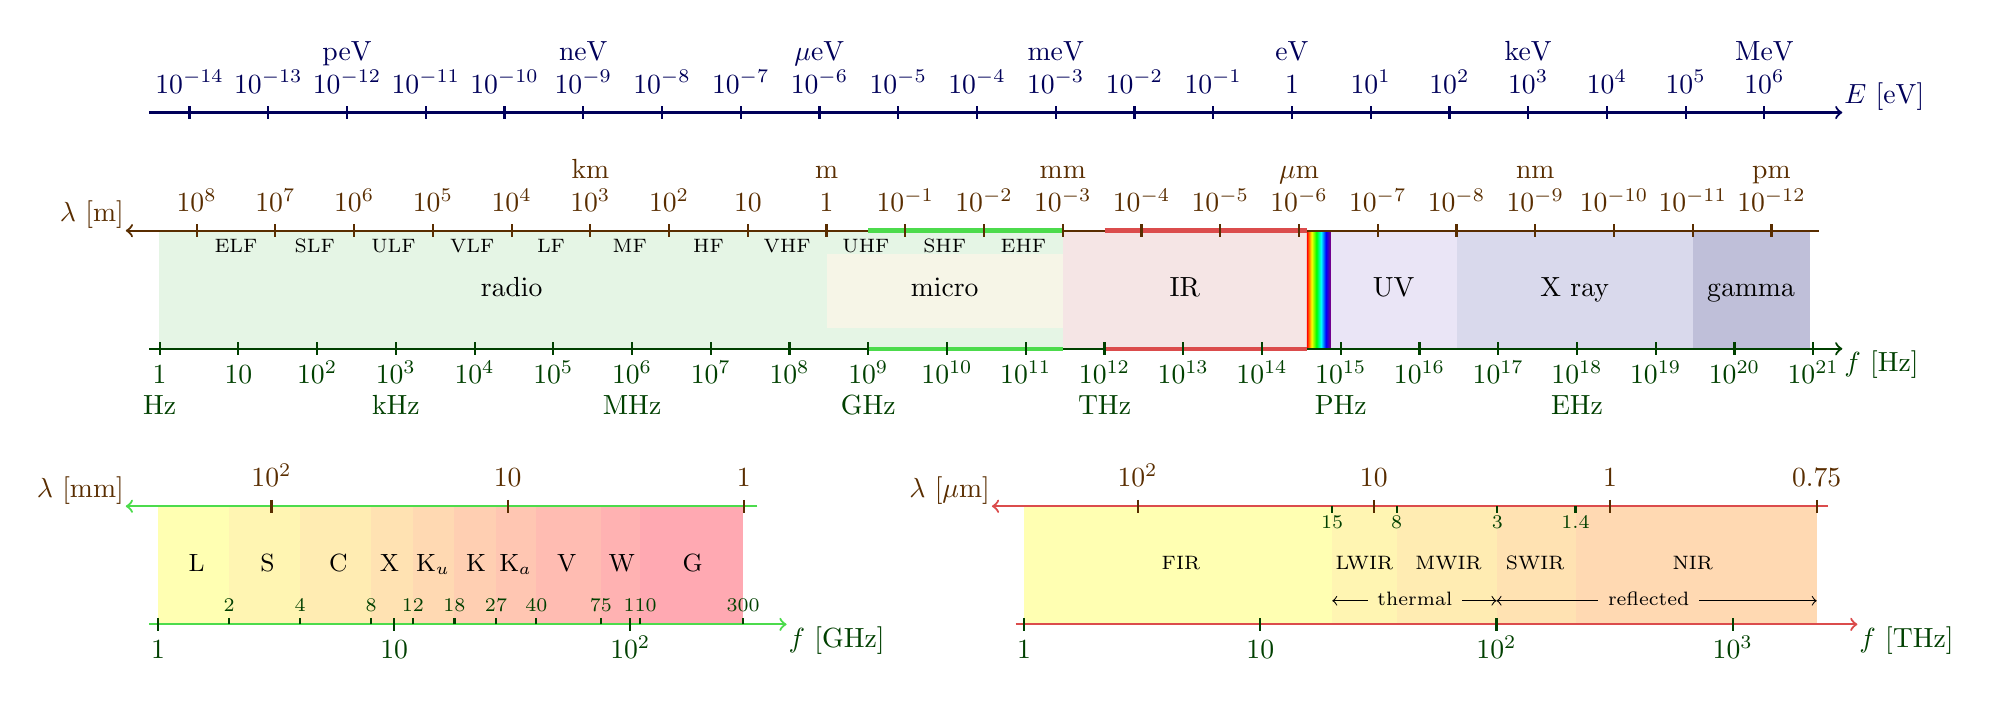
\begin{tikzpicture}

  \def\h{1.5}
  \def\radio{-8}
  \def\micro{0}
  \def\IR{3}
  \def\red{6.10}  % log(700e-9) = -6.15490196
  \def\blue{6.40} % log(400e-9) = -6.39794001
  \def\UV{6.40}
  \def\Xray{8}
  \def\gamm{11}
  \def\last{12}
  \def\radiof{-9}
  \def\dx{0.6}
  \def\yE{-\h}

  \def\tick#1#2#3{\draw[thick,#2] (#1+.08) --++ (0,-.16) node[below=-2pt,scale=1] {\strut #3};}
  \def\ticka#1#2#3{\draw[thick,#2] (#1+.08) --++ (0,-.16) node[above=2pt,scale=1] {\strut #3};}

  % MIDDLE
  \fill[green!60!black!10] (\radio-0.8*\dx,0) rectangle (\IR,\h);
  \fill[yellow!60!black!10] (\micro,0.18*\h) rectangle (\IR,0.8*\h);
  \fill[red!60!black!10] (\IR,0) rectangle (\red,\h);
  \fill[blue!60!violet!80!black!10] (\UV,0) rectangle (\Xray,\h);
  \fill[blue!50!black!15] (\Xray,0) rectangle (\gamm,\h);
  \fill[blue!40!black!25] (\gamm,0) rectangle (\last+0.82*\dx,\h);
  \shade[shading=rainbow,shading angle=-90] (\red,0) rectangle (\blue,\h);
  \node at ({(\radio+\micro)/2},\h/2) {\strut radio};
  \node at ({(\micro+\IR)/2},   \h/2) {\strut micro};
  \node at ({(\IR+\red)/2},     \h/2) {\strut IR};
  %\node at (\red,  \h/2) {red};
  %\node at (\red,  \h/2) {blue};
  \node at ({(\UV+\Xray)/2},    \h/2) {\strut UV};
  \node at ({(\Xray+\gamm)/2},  \h/2) {\strut X ray};
  \node at ({(\gamm+\last+0.8*\dx)/2},  \h/2) {\strut gamma};

  % WAVELENGTH
  \draw[->,thick,wavecol] (\last+\dx,\h) -- (\radio-1.5*\dx,\h) node[above left=-3] {$\lambda$ [\si{m}]};
  \draw[ultra thick, radarcol] (-8.47 + 9, \h) -- (3, \h);
  \draw[ultra thick, ircol] (-8.47+12, \h) -- (\red, \h);
  \foreach \x [evaluate={\i=int(-\x)}] in {\radio,...,\last}{
      \ifthenelse{\i=0}{ \ticka{\x,\h}{wavecol}{$1$} }
      { \ifthenelse{\i=1}{\ticka{\x,\h}{wavecol}{$10$}}
        {\ticka{\x,\h}{wavecol}{$10^{\i}$}} }
    }
  \node[wavecol,scale=1] at (-3,1.5*\h) {\strut km};
  \node[wavecol,scale=1] at ( 0,1.5*\h) {\strut m};
  \node[wavecol,scale=1] at ( 3,1.5*\h) {\strut mm};
  \node[wavecol,scale=1] at ( 6,1.5*\h) {\strut \si{\mu m}};
  \node[wavecol,scale=1] at ( 9,1.5*\h) {\strut nm};
  \node[wavecol,scale=1] at (12,1.5*\h) {\strut pm};
  %\node[wavecol,scale=1] at (15,1.71*\h) {\strut am};

  % FREQUENCY
  % log(f) = log(c) - log(lambda)
  % log(c) = log(2.997e8) = 8.4766867429
  \draw[->,thick,freqcol] (\radio-\dx,0) -- (\last+1.5*\dx,0) node[below right=-3] {$f$ [\si{Hz}]};
  \draw[ultra thick, radarcol] (-8.47 + 9, 0) -- (3, 0);
  \draw[ultra thick, ircol] (-8.47+12, 0) -- (\red, 0);
  \foreach \x [evaluate={\i=int(\x+9);\X=\x+0.53}] in {\radiof,...,\last}{
      \ifthenelse{\i=0}{\tick{\X,0}{freqcol}{$1$}}%
      {\ifthenelse{\i=1}{\tick{\X,0}{freqcol}{$10$}}
        {\tick{\X,0}{freqcol}{$10^{\i}$}}}
    }
  \node[freqcol,scale=1] at (-8.47,-0.5*\h) {\strut Hz};
  \node[freqcol,scale=1] at (-8.47+ 3,-0.5*\h) {\strut kHz};
  \node[freqcol,scale=1] at (-8.47+ 6,-0.5*\h) {\strut MHz};
  \node[freqcol,scale=1] at (-8.47+ 9,-0.5*\h) {\strut GHz};
  \node[freqcol,scale=1] at (-8.47+12,-0.5*\h) {\strut THz};
  \node[freqcol,scale=1] at (-8.47+15,-0.5*\h) {\strut PHz};
  \node[freqcol,scale=1] at (-8.47+18,-0.5*\h) {\strut EHz};

  % RADIO ITU BANDS
  \node at (-8.5 + 1, 0.85*\h) {\scriptsize \strut ELF};
  \node at (-8.5 + 2, 0.85*\h) {\scriptsize \strut SLF};
  \node at (-8.5 + 3, 0.85*\h) {\scriptsize \strut ULF};
  \node at (-8.5 + 4, 0.85*\h) {\scriptsize \strut VLF};
  \node at (-8.5 + 5, 0.85*\h) {\scriptsize \strut LF};
  \node at (-8.5 + 6, 0.85*\h) {\scriptsize \strut MF};
  \node at (-8.5 + 7, 0.85*\h) {\scriptsize \strut HF};
  \node at (-8.5 + 8, 0.85*\h) {\scriptsize \strut VHF};
  \node at (-8.5 + 9, 0.85*\h) {\scriptsize \strut UHF};
  \node at (-8.5 + 10, 0.85*\h) {\scriptsize \strut SHF};
  \node at (-8.5 + 11, 0.85*\h) {\scriptsize \strut EHF};

  % ENERGY
  % log(E) = log(hc) - log(lambda)
  % log(hc) = log(2.997e8*4.135e-15) = -5.9068377432
  \begin{scope}[shift={(0, 3)}]
    \draw[->,thick,enercol] (\radio-\dx,0) -- (\last+1.5*\dx,0) node[above right=-3] {$E$ [\si{eV}]};
    \foreach \x [evaluate={\i=int(\x-6);\X=\x-0.09}] in {\radio,...,\last}{
        \ifthenelse{\i=0}{ \ticka{\X,0}{enercol}{$1$} }
        { \ticka{\X,0}{enercol}{$10^{\i}$} }
      }
    %\node[enercol,scale=1] at (5.91-15,\yE-0.69*\h) {\strut feV};
    \node[enercol,scale=1] at (5.91-12,0.5*\h) {\strut peV};
    \node[enercol,scale=1] at (5.91- 9,0.5*\h) {\strut neV};
    \node[enercol,scale=1] at (5.91- 6,0.5*\h) {\strut \si{\mu eV}};
    \node[enercol,scale=1] at (5.91- 3,0.5*\h) {\strut meV};
    \node[enercol,scale=1] at (5.91+ 0,0.5*\h) {\strut  eV};
    \node[enercol,scale=1] at (5.91+ 3,0.5*\h) {\strut keV};
    \node[enercol,scale=1] at (5.91+ 6,0.5*\h) {\strut MeV};
    %\node[enercol,scale=1] at (5.91+9,\yE-0.69*\h) {\strut GeV};
  \end{scope}

  % Radar bands
  \begin{scope}[shift={(-8, -3.5)}]
    \def\radarend{7}
    \def\lastradar{2}

    \definecolorseries{rdr}{rgb}{last}{yellow!30}{red!30}
    \resetcolorseries{rdr}

    \foreach \i\j in {1/2, 2/4, 4/8, 8/12, 12/18, 18/27, 27/40, 40/75, 75/110, 110/300}{
        \fill[rdr!!+] ({3*log10(\i)-0.82*\dx}, 0) rectangle ({3*log10(\j)-0.82*\dx}, \h);
      }

    \node at (0, \h/2) {\small \strut L};
    \node at (.9, \h/2) {\small \strut S};
    \node at (1.8, \h/2) {\small \strut C};
    \node at (2.45, \h/2) {\small \strut X};
    \node at (3, \h/2) {\small \strut $\mathrm{K}_u$};
    \node at (3.55, \h/2) {\small \strut K};
    \node at (4.05, \h/2) {\small \strut $\mathrm{K}_a$};
    \node at (4.7, \h/2) {\small \strut V};
    \node at (5.4, \h/2) {\small \strut W};
    \node at (6.3, \h/2) {\small \strut G};

    \draw[->,thick,radarcol] (\radarend+0.2*\dx, \h) -- (-1.5*\dx, \h)%
    node[above left=-3,color=wavecol] {$\lambda$ [\si{mm}]};

    \foreach \x [evaluate={\i=int(2-\x); \j=int(\x); \X=\x+2*\j+.95}] in {0,...,\lastradar}{
        \ifthenelse{\i=0}{ \ticka{\X, \h}{wavecol}{$1$} }
        { \ifthenelse{\i=1}{\ticka{\X, \h}{wavecol}{$10$}}
          {\ticka{\X, \h}{wavecol}{$10^{\i}$}} }
      }

    \draw[->,thick,radarcol] (-\dx, 0) -- (\radarend+0.82*\dx, 0)%
    node[below right=-3,color=freqcol] {$f$ [\si{GHz}]};

    \foreach \x [evaluate={\i=int(\x); \X=\x+2*\i-0.82*\dx}] in {0, ..., \lastradar}{
        \ifthenelse{\i=0}{\tick{\X, 0}{freqcol}{$1$}}
        {\ifthenelse{\i=1}{\tick{\X, 0}{freqcol}{$10$}}
          {\tick{\X, 0}{freqcol}{$10^{\i}$}}}
      }

    % Intermediate ticks
    \foreach \f in {2, 4, 8, 12, 18, 27, 40, 75, 110, 300}{
        \draw[thick, freqcol] ({3*log10(\f)-0.82*\dx}, 0) -- ++(0,.08)%
        node[yshift=4pt, scale=1] {\scriptsize \strut \f};
      }

  \end{scope}

  % IR bands
  \begin{scope}[shift={(3, -3.5)}]
    \def\radarend{9.6}
    \def\lastradar{2}
    \def\lastradarf{3}

    %\ticka{-0.82*\dx, \h}{wavecol}{$1000$}

    %\foreach \i [evaluate={\x=(18-\i)/2}] in {15, 8, 3, 1.4, 0.7}{
    %    \ticka{\x-0.82*\dx, \h}{wavecol}{$\i$}
    %}

    \definecolorseries{ir}{rgb}{last}{yellow!30}{red!30}
    \resetcolorseries{ir}
    \fill[ir!!+] (-0.82*\dx, 0) rectangle ({6.95-3*log10(15)}, \h);
    \fill[ir!!+] ({6.95-3*log10(15)}, 0) rectangle ({6.95-3*log10(8)}, \h);
    \fill[ir!!+] ({6.95-3*log10(8)}, 0) rectangle ({6.95-3*log10(3)}, \h);
    \fill[ir!!+] ({6.95-3*log10(3)}, 0) rectangle ({6.95-3*log10(1.4)}, \h);
    \fill[ir!!+] ({6.95-3*log10(1.4)}, 0) rectangle ({6.95+3*log10(7.5)}, \h);

    \node at (1.5, \h/2) {\scriptsize \strut FIR};
    \node at (3.83, \h/2) {\scriptsize \strut LWIR};
    \node at (4.9, \h/2) {\scriptsize \strut MWIR};
    \node at (6, \h/2) {\scriptsize \strut SWIR};
    \node at (8, \h/2) {\scriptsize \strut NIR};

    \draw[->,thick,ircol] (\radarend+0.2*\dx, \h) -- (-1.5*\dx, \h)%
    node[above left=-3,color=wavecol] {$\lambda$ [\si{\mu m}]};

    \foreach \x [evaluate={\i=int(2-\x); \j=int(\x); \X=\x+2*\j+.95}] in {0,...,\lastradar}{
        \ifthenelse{\i=0}{ \ticka{\X, \h}{wavecol}{$1$} }
        { \ifthenelse{\i=1}{\ticka{\X, \h}{wavecol}{$10$}}
          {\ticka{\X, \h}{wavecol}{$10^{\i}$}} }
      }

    \ticka{{6.95+3*log10(7.5)}, \h}{wavecol}{$0.75$}

    \draw[->,thick,ircol] (-\dx, 0) -- (\radarend+0.82*\dx, 0)%
    node[below right=-3,color=freqcol] {$f$ [\si{THz}]};

    \foreach \x [evaluate={\i=int(\x); \X=\x+2*\i-0.82*\dx}] in {0, ..., \lastradarf}{
        \ifthenelse{\i=0}{\tick{\X, 0}{freqcol}{$1$}}
        {\ifthenelse{\i=1}{\tick{\X, 0}{freqcol}{$10$}}
          {\tick{\X, 0}{freqcol}{$10^{\i}$}}}
      }

    % Intermediate ticks
    \foreach \f in {1.4, 3, 8, 15}{
        \draw[thick, freqcol] ({6.95-3*log10(\f)}, \h) -- ++(0,-.08)%
        node[yshift=-4pt, scale=1] {\scriptsize \strut \f};
      }

    \draw[<-] (6-0.82*\dx, 0.2*\h) -- (6.8, 0.2*\h) node[anchor=west] (tmp) {\scriptsize \strut reflected};
    \draw[->] (tmp) -- ({6.95+3*log10(7.5)}, 0.2*\h);

    \draw[<-] ({6.95-3*log10(15)}, 0.2*\h) -- ++(0.45, 0) node[anchor=west] (tmp) {\scriptsize \strut thermal};
    \draw[->] (tmp) -- (6-0.82*\dx, 0.2*\h);

  \end{scope}

\end{tikzpicture}
\end{document}